\documentclass[pdf]{beamer}
\mode<presentation>{}
\usepackage{minted}
\usepackage{tikz}
\usepackage{pgffor} %% gives looping with \foreach
\usepackage[absolute,overlay]{textpos}
\usepackage{lmodern} %% scalable latin characters
\usetikzlibrary{arrows,shapes,backgrounds}
\usepackage{multirow}
\usepackage{listings} %% another package for code related stuff

%% stuff for minted
\definecolor{mintedBg}{rgb}{0.95, 0.95, 0.95}
\definecolor{blockBg}{rgb}{0.6, 0.6, 0.95}
\definecolor{rnaColor}{rgb}{0, 0.6, 0}
\definecolor{cdsColor}{rgb}{0, 0.4, 0.4}
\definecolor{rnaPol}{rgb}{0.8,0,0.8}
\definecolor{ribosomeCol}{rgb}{0.5,0.5,0.1}
\definecolor{protColor}{rgb}{0.6,0,0.6}
%% colours for nucleotides:
\definecolor{dACol}{rgb}{0.5, 0.5, 0}
\definecolor{dCCol}{rgb}{0.8, 0, 0}
\definecolor{dGCol}{rgb}{0, 0.8, 0}
\definecolor{dTCol}{rgb}{0, 0, 0.8}
    
%% define styles for different codes
\newminted{cpp}{linenos, bgcolor=blockBg, fontsize=\footnotesize}
%% then use \begin{cppcode}
\newminted{c}{linenos, bgcolor=mintedBg, fontsize=\footnotesize}
\newminted{perl}{linenos, bgcolor=mintedBg, fontsize=\footnotesize}

%% a command to define a subheading
\newcommand\subHeading[1]{
  \par\bigskip {\Large\bfseries#1}\par\smallskip
}

%% I detest indentation in footnotes etc, so try this:
\makeatletter
\renewcommand\@makefntext[1]{\noindent\makebox[0em][r]{\@makefnmark}\tiny#1}
\makeatother
%% the makeatletter and makeatother are required to allow me to
%% to change the macro beginning with an @. (though when I call it
%% I don't use the @ ... 

\setlength\parskip{0.5em}
\setlength\parindent{0ex}

%% to have footnotes without references. This from tex.stackexchange.com
\newcommand\blfootnote[1]{%
  \begingroup  %% this makes it a local redefinition
  \renewcommand\thefootnote{}\footnote{#1}%
  \addtocounter{footnote}{-1}  % this adjusts the footnote counter
  \endgroup
}


\title{Bioinformatics: the problem domain}
\subtitle{Fields in Bioinformatics}
\author{Martin Jakt}

\begin{document}

\begin{frame}
  \titlepage
\end{frame}

\begin{frame}{Problems and fields in Bioinformatics}
  \small
  Any problem that involves the processing of biological information.\footnote
  {Strictly speaking, does not need to involve computers, but usually does}

  \begin{description}[Sequence alignment]
    \item<2->[Phylogeny] Based on quantification of differences between objects (which
      may be sequences).
    \item<3->[Sequence analysis] Properties and transformations of sequences (eg. translation)
    \item<4->[Sequence alignment] Required for many (most?) other types of analyses.
    \item<5->[Omics] Big data analysis, usually related to:
      \begin{itemize}
        \item<5-> DNA sequence assembly and annotation
        \item<5-> Gene expression (transcript abundancies)
        \item<5-> Chromatin state (DNA methylation and histone modification)
        \item<5-> Sequence variation (between individuals / strains / cells)
      \end{itemize}
    \item<6->[Databases] Development of databases that facilitate storage, lookup and analysis.
    \item<7->[Structures] Prediction of protein and RNA structures.
      Difficult\footnote{More physics than informatics}.
  \end{description}

\end{frame}

\begin{frame}{Why sequence analysis?}
  \begin{enumerate}
    \item Genetic information is encoded as a sequence of bases.
    \item Technically easy to obtain sequence information (DNA sequencing).
    \item Provides digital or qualitative information (i.e. we can define
      identities, and establish causal relationships).
    \item Easier than describing biochemical activities (quantitative information
      from difficult experiments).
  \end{enumerate}
  \uncover<2>{
    It's a cheap way to get lots of biological information.

    A means to perform other types of analyses.
  }
\end{frame}

\begin{frame}{Biochemistry before cheap sequencing}
  %% lets make a tikz picture
  \begin{figure}[ht]
    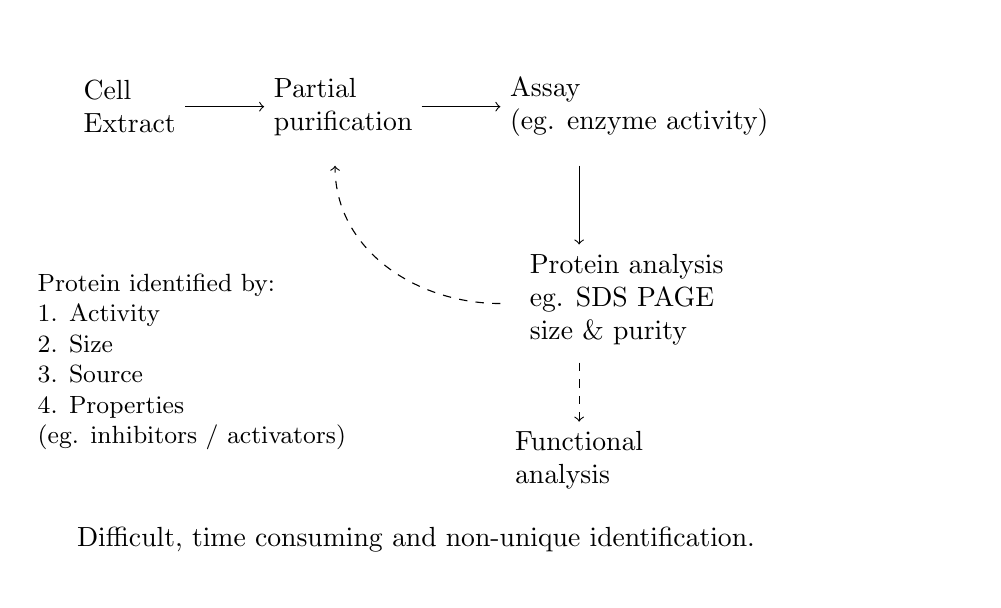
\begin{tikzpicture}[scale=0.5]
      \draw [help lines, opacity=0] (0,0) grid (24,14);
      %\foreach \x in {1,2,...,22} \node [font=\small] at (\x,1) {\x};
      %\foreach \y in {1,2,...,14} \node [font=\small] at (23,\y) {\y};
      \node [left, align=left] at (4,12) {Cell\\Extract};
      \pause
      \draw [->] (4,12) -- (6,12) node [right, align=left] {Partial\\purification};
      \pause
      \draw [->] (10,12) -- (12,12) node [right, align=left] {Assay\\(eg. enzyme activity)};
      \pause
      \draw [->] (14,10.5) -- (14,8.5);
      \node [below right, align=left] at (12.5,8.5) {Protein analysis\\eg. SDS PAGE\\size \& purity};
      \pause
      \draw [->,dashed] (12,7) to [out=180,in=270] (7.8,10.5);
      \pause
      \draw [->,dashed] (14,5.5) -- (14,4) node [below, align=left] {Functional\\analysis};
      \pause
      \node [below right, align=left, font=\small] at (0,8) {Protein identified by:\\1. Activity\\2. Size\\
        3. Source\\4. Properties\\  (eg. inhibitors / activators)};
      \pause
      \node [right] at (1,1) {Difficult, time consuming and non-unique identification.};
    \end{tikzpicture}
  \end{figure}
\end{frame}

\begin{frame}{Molecular biology before cheap sequencing}
  \begin{figure}[ht]
    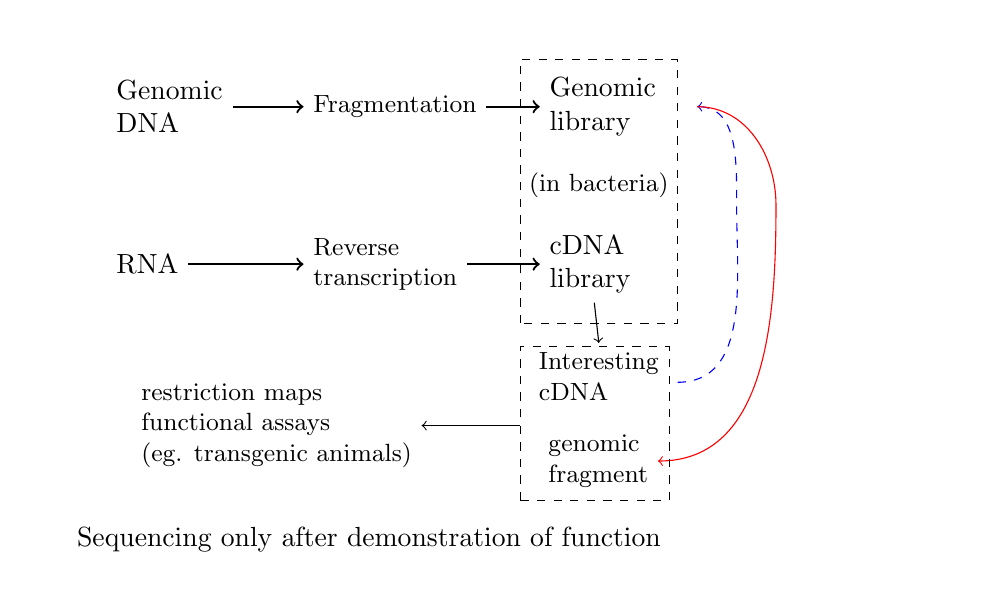
\begin{tikzpicture}[scale=0.5]
      \draw [help lines, opacity=0] (0,0) grid (24,14);
%      \foreach \x in {1,2,...,22} \node [font=\small] at (\x,1) {\x};
%      \foreach \y in {1,2,...,14} \node [font=\small] at (23,\y) {\y};
      \node [right, align=left] (gdna) at (2,12) {Genomic\\DNA};
      \node [right, align=left, dashed, font=\small] (frag) at (7,12) {Fragmentation};
      \node [right, align=left] (glib) at (13,12) {Genomic\\library};
      \node [right, align=left] (rna) at (2,8) {RNA};
      \node [right, align=left, dashed, font=\small] (rtran) at (7,8) {Reverse\\transcription};
      \node [right, align=left] (cdlib) at (13,8) {cDNA\\library};
      \draw [->, thick] (gdna) -- (frag);
      \draw [->, thick] (frag) -- (glib);
      \draw [->, thick] (rna) -- (rtran);
      \draw [->, thick] (rtran) -- (cdlib);
      \draw [dashed] (12.5,6.5) rectangle (16.5,13.2);
      \node [font=\small] at (14.5,10) {(in bacteria)};
      \pause
      \draw [->] (cdlib) -- (14.5,6) node [below, align=left, font=\small] 
      {Interesting\\cDNA};
      \pause
      \draw [->, dashed, blue] (16.5,5) to [out=0,in=270] (18,9.5) to
      [out=90,in=0] (17,12);
      \draw [->, red] (17,12) to [out=0,in=90] (19,9.5) to
      [out=270,in=0] (16,3) node [left, align=left, font=\small, black] 
      {genomic\\fragment};
      \pause
      \draw [dashed] (12.5,2) rectangle (16.3,5.9);
      \draw [->] (12.5,3.9) -- (10,3.9) node [left, align=left, font=\small]
      {restriction maps\\functional assays\\(eg. transgenic animals)};
      \pause
      \node [right] at (1,1) {Sequencing only after demonstration of function};
    \end{tikzpicture}
  \end{figure}
\end{frame}

\begin{frame}{Genetics before cheap sequencing}
  %% lets make a tikz picture
  \begin{figure}[ht]
    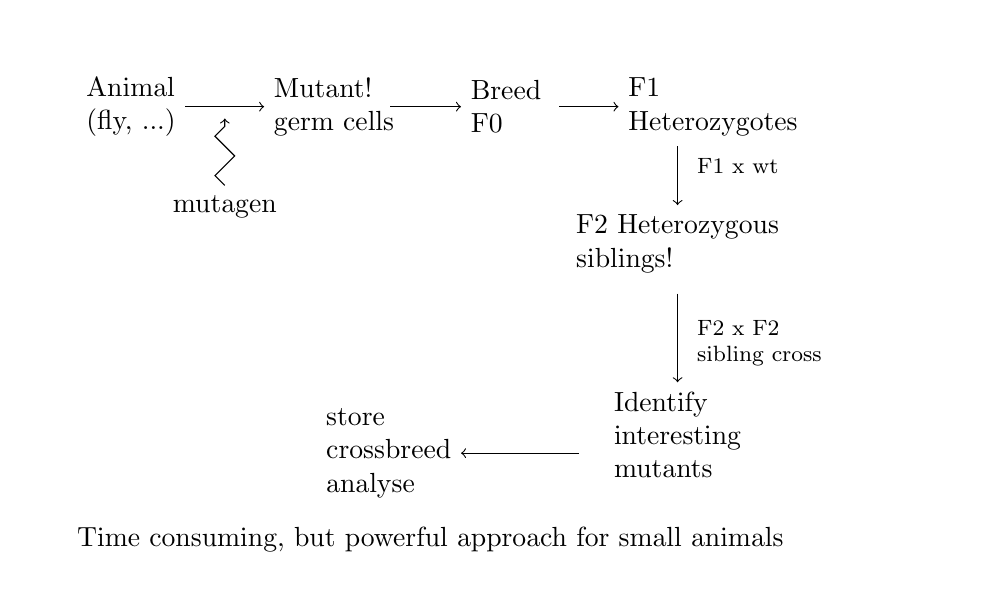
\begin{tikzpicture}[scale=0.5]
      \draw [help lines, opacity=0] (0,0) grid (24,14);
      %\foreach \x in {1,2,...,22} \node [font=\small] at (\x,1) {\x};
      %\foreach \y in {1,2,...,14} \node [font=\small] at (23,\y) {\y};
      \node [left, align=left] at (4,12) {Animal\\(fly, ...)};
      \pause
      \draw [->] (4,12) -- (6,12) node [right, align=left] {Mutant!\\germ cells};
      \draw [->] (5,10) node [below] {mutagen} -- (4.75,10.25) -- (5.25,10.75) -- 
      (4.75,11.25) -- (5,11.5) -- (5,11.7);
      \pause
      \draw [->] (9.2,12) -- (11,12) node [right, align=left] {Breed\\F0};
      \draw [->] (13.5,12) -- (15,12) node [right, align=left] {F1\\Heterozygotes};
      \draw [->] (16.5,11) -- (16.5, 9.5) node [below, align=left] {F2 Heterozygous\\siblings!};
      \node [right, font=\footnotesize] at (16.75, 10.5) {F1 x wt};
      \node [right, align=left, font=\footnotesize] at (16.75,6) {F2 x F2\\sibling cross};
      \draw [->] (16.5, 7.25) -- (16.5, 5) node [below,align=left] {Identify\\interesting\\mutants};
      \draw [->] (14,3.2) -- (11,3.2) node [left, align=left] {store\\crossbreed\\analyse};
      \pause
      \node [right] at (1,1) {Time consuming, but powerful approach for small animals};
    \end{tikzpicture}
  \end{figure}
\end{frame}

\begin{frame}{Identification of activities \& functions}
  Biochemical functions identified by:
  \begin{itemize}
    \item A functional assay (eg. phosphorylation of a substrate)
    \item A size on a gel (a single band being the holy grail)
    \item Other properties (eg. activators / repressors)
  \end{itemize}
  Genetic function identified by:
  \begin{itemize}
    \item Phenotype
    \item Relative location determined by breeding
  \end{itemize}
  Neither of these is very precise, and difficult to use across species.

  Sequence analysis allows cross-species comparisons and less ambiguous
  identification. 
  \pause
  \bf{Assigning identity is necessary to combine information from different sources} 
\end{frame}

\begin{frame}{Biochemistry \& genetics after cheap sequencing}
  \begin{itemize}
  \item Identify interesting genes from external data sources:
    \pause
    \begin{itemize}
    \item Sequence motifs indicating function
    \item Expression pattern (across cell types or experimental conditions)
    \item Mutation or genetic mapping indicating a functional role
    \item Literature
    \end{itemize}
    \pause
  \item Use sequence to make protein \& do biochemistry
  \item Use sequence to study expression and protein behaviour in detail
  \item Use sequence to remove or over-express gene in animals
  \item Use sequence to investigate the regulation of the gene
  \item Use sequence to investigate genetic origins of the gene
  \end{itemize}
  \pause
  Lots of ways of making use of sequence data. These are just examples.\\
  here: sequence $\equiv$ piece of DNA
\end{frame}

\begin{frame}{Sequence to protein biochemistry}
  %% lets make a tikz picture
  \begin{figure}[ht]
    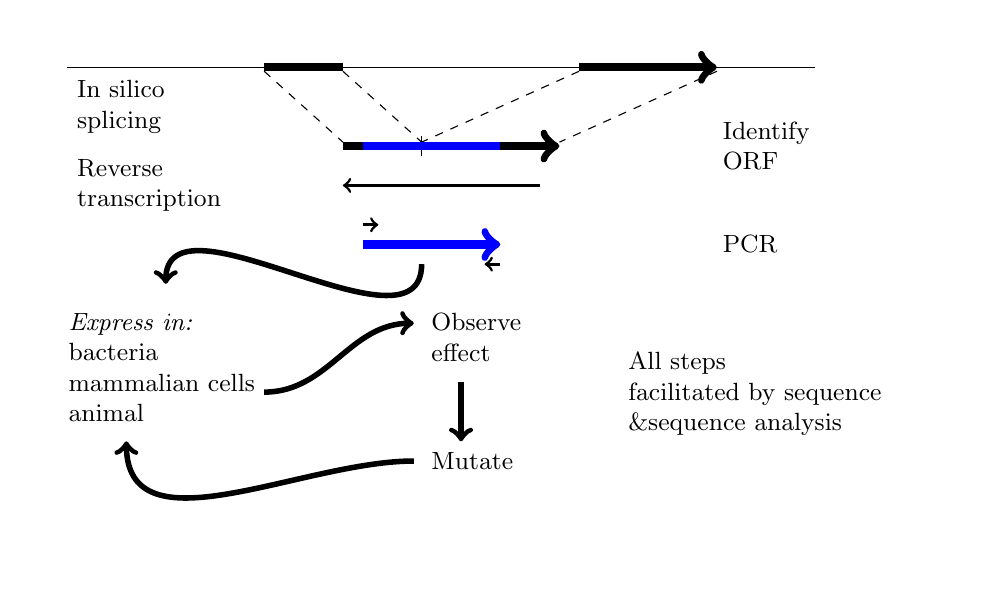
\begin{tikzpicture}[scale=0.5]
      \draw [help lines, opacity=0] (0,0) grid (24,14);
%      \foreach \x in {1,2,...,22} { \node [font=\small] at (\x,1) {\x}; }
%      \foreach \y in {1,2,...,14} \node [font=\small] at (23,\y) {\y};
      \draw [line width=0.5, -] (1,13) -- (20,13);
      \draw [line width=3, -] (2+4,13) -- (4+4,13);
      \draw [line width=3, ->] (10+4,13) -- (13.5+4,13);
      \visible<2->{
        \draw [line width=3, ->] (4+4,11) -- (9.5+4,11);
        \draw [-] (6+4,10.75) -- (6+4,11.25);
        \draw [-, dashed] (2+4,12.9) -- (4+4,11.1);
        \draw [-, dashed] (4+4,12.9) -- (6+4,11.1);
        \draw [-, dashed] (10+4,12.9) -- (6+4,11.1);
        \draw [-, dashed] (13.5+4,12.9) -- (9.5+4,11.1);
        \node [font=\small, right, align=left] at (1,12) {In silico\\splicing};
      }
      \visible<3->{
        \draw [line width=3, blue] (8.5,11) -- (12,11);
        \node [font=\small, right, align=left] at (17.4,11) {Identify\\ORF};
      }
      \visible<4->{
        \draw [line width=1, ->] (13,10) -- (8,10);
        \node [font=\small, right, align=left] at (1,10) {Reverse\\transcription};
      }
      \visible<5->{
        \draw [->, line width=1] (8.5,9) -- (8.9,9);
        \draw [->, blue, line width=3] (8.5,8.5) -- (12,8.5);
        \draw [->, line width=1] (12,8) -- (11.6,8);
        \node [font=\small, right, align=left] at (17.4,8.5) { PCR };
      }
      \visible<6->{
        \node [font=\small, below, align=left] at (3.4,7) {\emph{Express
          in:}\\bacteria\\mammalian cells\\animal};
        \draw [->, line width=2] (10,8) to [out=270,in=90] (3.5,7.5);
      }
      \visible<7->{
        \node [font=\small, below right, align=left] at (10,7) {Observe\\effect};
        \node [font=\small, right, align=left] at (10,3) {Mutate};
        \draw [->, line width=2] (6,4.75) to [out=0,in=180] (9.8,6.5);
        \draw [->, line width=2] (11,5) -- (11,3.5);
        \draw [->, line width=2] (9.8,3) to [out=180,in=270] (2.5,3.5);
      }
      \visible<8->{
        \node [font=\small, below right, align=left] at (15,6) {All
          steps\\facilitated by sequence\\\&sequence analysis};
      }
    \end{tikzpicture}
  \end{figure}
\end{frame}

\begin{frame}{Gene regulation}
  %% lets make a tikz picture
  \begin{figure}[ht]
    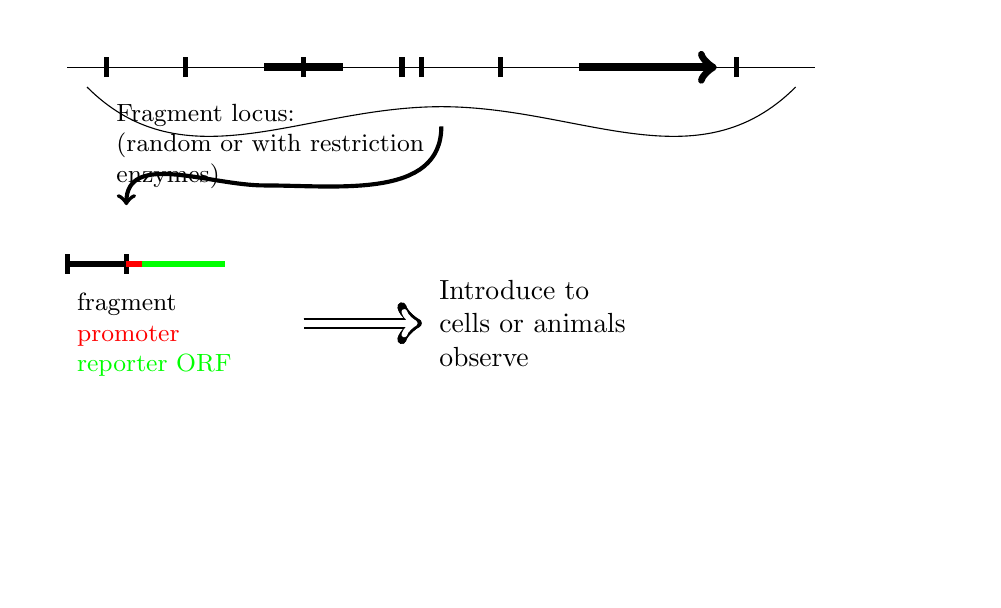
\begin{tikzpicture}[scale=0.5]
      \draw [help lines, opacity=0] (0,0) grid (24,14);
%      \foreach \x in {1,2,...,22} { \node [font=\small] at (\x,1) {\x}; }
%      \foreach \y in {1,2,...,14} \node [font=\small] at (23,\y) {\y};
      \draw [line width=0.5, -] (1,13) -- (20,13);
      \draw [line width=3, -] (2+4,13) -- (4+4,13);
      \draw [line width=3, ->] (10+4,13) -- (13.5+4,13);
      \def \xpos {2,4,7,9.5,10,12,18}
      \visible<2->{
        \foreach \x in \xpos  \draw [-, line width=2] (\x,12.75) --
        (\x,13.25); 
      }
      \visible<2>{
        \node [font=\small, right, align=left] at (2,11) 
              {Fragment locus:\\(random or with restriction\\enzymes)};
      }
      \visible<3->{
        \draw [-] (1.5,12.5) to [out=315,in=180] (10.5,12)
        to [out=0,in=225] (19.5,12.5);
        \draw [->, line width=1.5] (10.5,11.5) to [out=270,in=0] (6,10)
        to [out=180,in=90] (2.5,9.5);
        \draw [-, line width=2] (1,8) -- (2.5,8);
        \draw [-, line width=2] (1,8.25) -- (1,7.75);
        \draw [-, line width=2] (2.5,8.25) -- (2.5,7.75);
        \draw [-, line width=2, red] (2.5,8) -- (2.9,8);
        \draw [-, line width=2, green] (2.9,8) -- (5,8);
        \node [below right, align=left, font=\small] at (1,7.5)
        {fragment\\\textcolor{red}{promoter}\\\textcolor{green}{reporter
            ORF}};
        \draw [->, line width=4] (7,6.5) -- (10,6.5);
        \draw [->, line width=4] (7,6.5) -- (10,6.5);
        \draw [->, line width=2.5, white] (7,6.5) -- (9.9,6.5);
        \node [right, align=left] at (10.2,6.5) {Introduce to\\cells or animals\\observe};
%%        \arrow [thick] (8,6.5) -- (10,6.5);
      }
    \end{tikzpicture}
  \end{figure}
\end{frame}

\begin{frame}{Sequence use}
  In the two previous examples sequence data was primarily used to construct
  fragments of DNA that can be propagated, integrated or temporarily
  introduced to cells and animals (or plants).

  Very simple sequence analysis, based on identification of regions, sites and
  using these to work out how to cut, copy and paste DNA fragments around.

  But, done well, there would also be analyses to :
  \begin{itemize}
  \item Identify amino acids residues to mutate
  \item Identify conserved / non-conserved peptide fragments
  \item Identify conserved non-coding regions (likely to be regulatory)
  \item Make sense of active regions (i.e. identify interaction partners)
  \end{itemize}
  
\end{frame}

\begin{frame}{General sequence analysis}
  Not just alignments.
  \begin{figure}[ht]
    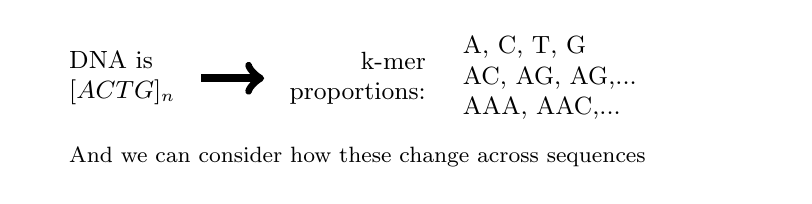
\begin{tikzpicture}[scale=0.4]
      \draw [help lines, opacity=0] (0,0) grid (24,3.5);
      %\foreach \x in {1,2,...,22} \node [font=\small] at (\x,0) {\x};
      %\foreach \y in {1,2,...,5} \node [font=\small] at (23,\y) {\y};
      \visible<2->{
        \node [right, align=left,font=\small] at (1,2.5) {DNA is\\$[A C T G]_n$};
      }
      \visible<3->{
        \draw [->, line width=3] (5.5,2.5) -- (7.5,2.5);
        \node [right, align=right, font=\small] at (8,2.5) {k-mer\\proportions:};
        \node [right, align=left, font=\small] at (13.5,2.5) {A, C, T, G\\AC, AG, AG,...\\AAA, AAC,...};
      }
      \visible<4->{
        \node [right, align=left, font=\footnotesize] at (1,0) {And we can consider how these change across sequences};
      }
      %% the following causes the above never to show
%      \visible<7->{ 
%        \node [left, font=\large] at (1,2) {All of these observations are related to interesting biological phenomena}; 
%      }
    \end{tikzpicture}
  \end{figure}
  \small
  \visible<5->{
    This seems like counting for the sake of counting. But
  }
  \visible<6->{
    \begin{enumerate}
    \item Genomes typically have less C and G than A and T (low CG/AT ratio)
    \item Regions containing high levels of the CG dinucleotide 
      are associated with many promoters (ca. 50\%)
    \item Thermophiles tend to have higher CG/AT ratios
    \end{enumerate}
  }
\end{frame}

\begin{frame}[fragile]{Sequence Alignment (1)}
  Why align sequences?
  
  \begin{itemize}
    \item Sequence assembly
    \item Sequence comparison
    \item Motif (structure) discovery
    \item ...
  \end{itemize}
  \pause
  Lots of uses, but for genomics, possibly the most important reason:

  It facilitates high-throughput analyses of gene expression and chromatin modification.
\end{frame}

\begin{frame}{Assembly?}
  \begin{itemize}
  \item DNA sequences are long...
    \begin{itemize}
    \item Eukaryotic chromosomes can be 100s of millions of bases
    \item Plasmids usually 3-10 thousand bases
    \end{itemize}
  \item Sequencing technology usually gives us short sequences
    \pause
    \begin{itemize}
    \item Traditional Sanger sequencing: 100 - 1000 bases
    \item First (ish) next generation sequencing (NGS) (454) $\sim$500 bases
    \item Next NGS (Solexa/Illumina) 30-50 bases
    \item Next next NGS (Illumina/SOLID/IonTorrent) $\sim$300-600 bases
    \item Newest NGS (PacBio/Nanopore) $\rightarrow$50,000 (?) bases
    \end{itemize}
  \end{itemize}
  Many short fragments have to be assembled to obtain useful sequence.
\end{frame}

%% we can't use \verbatim and \visible in the frame,
%% so we have to assemble them outside of the frame
\defverbatim{\assemblebox}{
\footnotesize
\linespread{0.65}
\begin{verbatim}
The s
    smel 
      ell: th
             at's
                s the first
                        rst thing t
                                g that hi
                                       hits you, p
                                                 
hits you, p
          promising ever
                      erything in ex
                                  exchange for
                                            or your soul
\end{verbatim}
}
 
\begin{frame}[fragile]{Sequence assembly}
\small
A piece of fragmented prose:

"exchange for" "hits you, p" "g that hi" 
"erything in ex" " smel" "ell: th"  
"or your soul" " promising ever" "rst thing t" "The s"  
"at's" "s the first" 

Reassemble:
\visible<2->{
\assemblebox
"The smell: that's the first thing that hits you, promising everything in exchange for your soul."\\
-- Graham Greene, The Quiet American 
}

\visible<3->{
%% overlay removes the picture from the ordinary page flow
%% and lets me draw on top of the text
\begin{tikzpicture}[overlay]
  \draw [help lines, opacity=0.0] (0,0) grid (13,8);
%  \foreach \x in {1,2,...,10} \node [font=\small] at (\x,0) {\x};
%  \foreach \y in {1,2,...,10} \node [font=\small] at (11,\y) {\y};

  \draw [-, red, thick] (2.17,5.2) -- (2.17,5.8);
\end{tikzpicture}
}
%\tiny
%"I can't say what made me fall in love with Vietnam - that a woman's voice can drug you; that everything is so intense. 
%The colors, the taste, even the rain. Nothing like the filthy rain in London. They say whatever you're looking for, 
%you will find here. They say you come to Vietnam and you understand a lot in a few minutes, but the rest has got to be 
%lived. The smell: that's the first thing that hits you, promising everything in exchange for your soul. And the heat. 
%Your shirt is straightaway a rag. You can hardly remember your name, or what you came to escape from. 
%But at night, there's a breeze. The river is beautiful. You could be forgiven for thinking there was no war; that the 
%gunshots were fireworks; that only pleasure matters. A pipe of opium, or the touch of a girl who might tell you she 
%loves you. And then, something happens, as you knew it would. And nothing can ever be the same again."\\

\end{frame}

\begin{frame}{Sequence assembly (2)}
  Assembly is difficult:
  \begin{itemize}
    \item Regions of low-complexity sequences (eg. AAAAAA$_x$)
    \item Presence of repeat sequences
    \item Regions with direct and inverted repeats
    \item Some DNA sequences can be difficult to amplify (either in bacteria
      or by PCR)
    \item The algorithmic complexity of comparing all fragments to all
      fragments
  \end{itemize}
  Genome assembly cannot usually be done completely from simple libraries of
  short fragments. Additional methods (eg. mate-pair libraries are also required).
\end{frame}

\defverbatim{\marvBox}{
\small
\linespread{0.8}
\begin{verbatim}
martin
|||*||
marvin
\end{verbatim}
}

\defverbatim{\maryBox}{
\small \linespread{0.8}
\begin{verbatim}
mar-y had a little lamb
||| |||||||||||||||||||
marty had a little lamb
\end{verbatim}
}

\begin{frame}{Sequence comparison(1)}
  Why bother?
  \begin{itemize}
    \item Infer evolutionary relationship (between and within species)
    \item Deduce function of a sequence
    \item Infer the presence of functional motifs (align lots of sequences,
      regions of high similarity suggest the presence of a function)
    \item ...
  \end{itemize}
  
\end{frame}

\begin{frame}{Sequence comparison (2)}
  Consider the similarity between the two following sequences:
  \begin{enumerate}
    \item martin
    \item marvin
  \end{enumerate}
  \visible<2->{ \marvBox }
  \visible<3->{
      Similarity: 5 matches / 6 positions.
      Very simple, because aligned.
  }
  \visible<4->{
  But:
  \begin{enumerate}
    \item mary had a little lamb
    \item marty had a little lamb
  \end{enumerate}
  }
  \visible<5->{ \maryBox 
    Similarity: 22/23 but must be aligned first.
  }
  
\end{frame}

\begin{frame}{Sequence Identification}
  Searching a database.

  A partial sequence identified by some means:
  \begin{enumerate}
    \item Protein purified and partial amino acid sequence determined.
    \item A small RNA tag identified as specifically expressed.
    \item A number of sequences obtained that associate with a given protein.
    \item A sequence identified by expression cloning that encodes a protein with
      a specific function.
    \item A sequence identified that can direct the expression of a reporter gene
      in a specific cell type.
    \item ...
  \end{enumerate}
\end{frame}

\begin{frame}{continued...}
  These represent:
  \begin{description}
  \item[1,2,4] Partial RNA or protein sequences.
  \item[3,5] Sequences marking specific locations in the genome.
    
  \end{description}
  \visible<2->{
    For these we would wish to:
    \begin{description}
    \item[1,2,4] Obtain the remainder of the sequence and determine what is known
      about the protein or RNA encoded by the sequence.
    \item[3,5] Find the location of the sequence in the genome and determine what
      genes may be associated with it.
    \end{description}
  }
  \visible<3->{
    i.e. we wish to align our sequences to all known sequences.\\
    Amazingly, this is not difficult!
  }
\end{frame}

\begin{frame}{Sequence alignment}
  Alignment of sequences underpins a very large proportion of analyses at some point,

  \pause
  ..., and will consequently be covered in some detail.

\end{frame}

\begin{frame}{Omics}
  The study of complete things (eg. complete genomes).
  \pause
  or more frequently:\\
  \hspace{2em}the analysis of any large biological data set.
  %% note the use of pseudo to have blank space as well. Good to
  %% remember.
  \pause
  \begin{description}[Transcriptomics]
  \item[Genomics] Properties of genomes.
  \item[Transcriptomics] Parallel measurements of the abundancies of all\footnote{well, almost all} transcripts.
  \item[Proteomics] Parallel estimates of the abundancies of lots\footnote{all proteins, too difficult} of proteins.
  \item[epigenomics?] Measurements of the chromatin state (histone modifications, DNA methylations, etc..) across the whole genome.
  \end{description}
  All these generate large amounts of data that must be analysed to provide
  any insights.

\end{frame}

\begin{frame}{Omics (2)}
  \begin{itemize}
    \item Transcriptomics
    \item Proteomics
    \item Epigenomics
    \item ...
  \end{itemize}
  Usually referred to as:
  functional genomics\footnote{mostly a branding exercise}

\end{frame}

\begin{frame}{Genomics?}
  \begin{figure}[ht]
    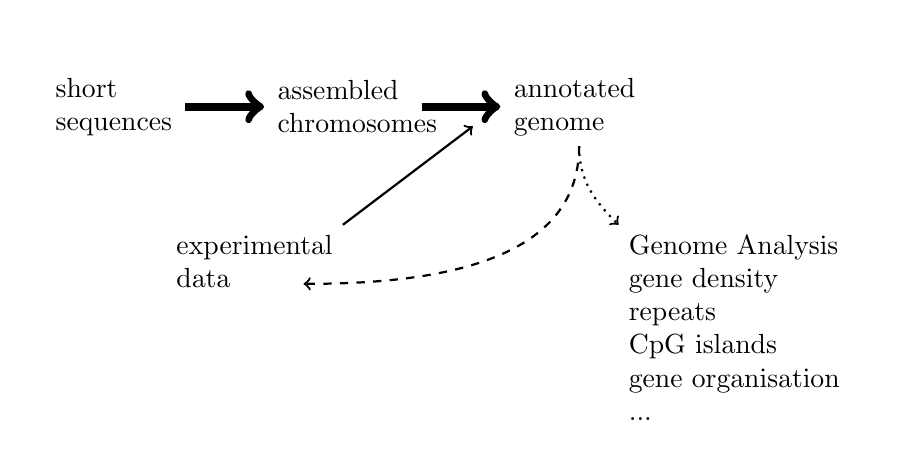
\begin{tikzpicture}[scale=0.5]
      \draw [help lines, opacity=0] (0,0) grid (22,10);
      %\foreach \x in {1,2,...,19} \node [font=\small] at (\x,0) {\x};
      %\foreach \y in {1,2,...,10} \node [font=\small] at (20,\y) {\y};
      \draw [->, line width=3] (4,8) node [left, align=left] { short\\sequences }
      -- (6,8) node [right, align=left] {assembled\\chromosomes};
      \draw [->, line width=3] (10,8) -- (12,8) node [right, align=left]
      {annotated\\genome};
      \draw [->, thick] (8,5) node [below left, align=left] {experimental\\data}
      -- (11.3,7.5);
      \draw [->, thick, dashed] (14,7) to [out=270,in=0] (7,3.5);
      \draw [->, thick, dotted] (14,7) to [out=270,in=135] (15,5) node 
      [below right, align=left] {Genome Analysis\\gene density\\repeats\\CpG islands\\gene organisation\\...};

    \end{tikzpicture}
  \end{figure}
\end{frame}

\begin{frame}{Genomics questions}
  \begin{itemize}
    \pause
  \item How many genes?
    \pause
  \item How much intergenic space?
    \pause
  \item How repetitive?
    \pause
  \item Intron / exon size distributions.
    \pause
  \item How variable between individuals (i.e. population genetics)?
    \pause
  \item How divergent from related species?
    \pause
  \item CpG density.
    \pause
  \item Evolutionary origins (eg. genome duplications, etc..)
    \pause
  \item Frequence of horizontal gene transfer.
    \item ...
  \end{itemize}
\end{frame}

\begin{frame}{Transcriptomics (1)}
  Expression values from:
  \begin{itemize}
    \item Serial Expression of Gene Expression (SAGE) (old method).
    \item DNA microarrays.
    \item Next generation sequencing (newest method).
  \end{itemize}
  What are we looking for?
  \begin{itemize}
    \item Data structure
    \item Correlations within the data (gene-gene and sample-sample)
    \item Correlations with sample factors
      \begin{itemize}
        \item General correlations (eg. activation of specific classes of genes)
        \item Individual genes (i.e. data mining)
      \end{itemize}
    \item Correlation with external data (eg. DNA sequence)
  \end{itemize}
\end{frame}

\begin{frame}{Transcriptomics (2)}
  Genome wide expression patterns by NGS:
  \begin{figure}[ht]
    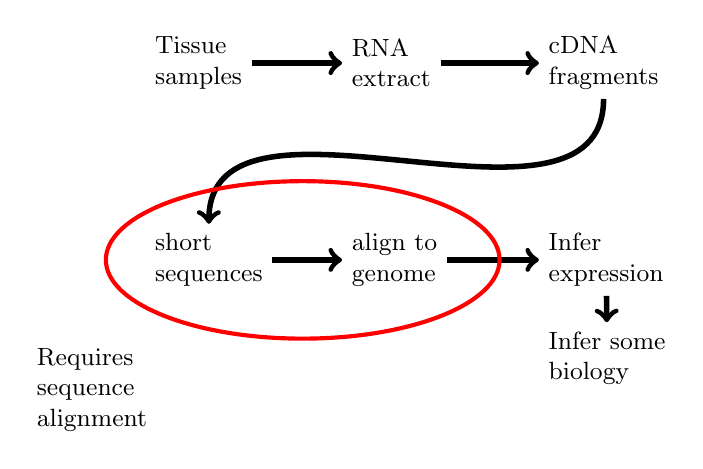
\begin{tikzpicture}[scale=0.5]
      %% \draw [help lines, opacity=0.5] (0,0) grid (20,10);
      %% \foreach \x in {1,2,...,19} \node [font=\small] at (\x,0) {\x};
      %% \foreach \y in {1,2,...,10} \node [font=\small] at (20,\y) {\y};

      \node [right, align=left, font=\small] (a) at (1,10) {Tissue\\samples};
      \node [right, align=left, font=\small] (b) at (6,10) {RNA\\extract};
      \node [right, align=left, font=\small] (c) at (11,10) {cDNA\\fragments};
      \draw [->, line width=2] (a) -- (b);
      \draw [->, line width=2] (b) -- (c);
      
      \visible<2->{
        \node [right, align=left, font=\small] (d) at (1,5) {short\\sequences};
        \node [right, align=left, font=\small] (e) at (6,5) {align
          to\\genome};
        \node [right, align=left, font=\small] (f) at (11,5) {Infer\\expression};
        \draw [->, line width=2] (c) to [out=270,in=90] (d);
        \draw [->, line width=2] (d) to (e);
        \draw [->, line width=2] (e) to (f);
      }
      \visible<3->{
        \node [right, align=left, font=\small] (g) at (11,2.5) {Infer
          some\\biology};
        \draw [->, line width=2] (f) -- (g);
      }
      \visible<4->{
        \draw [line width=1.5, red] (5,5) ellipse (5 and 2);
        \node [below right, align=left, font=\small] at (-2,3) {Requires\\sequence\\alignment};
      } 

%%       \node [above] at (10,9) {Samples};
%%       \node [above, rotate=90] at (1,5) {Genes};
%% %      \draw [->] (9,8.75) node [left, font=\footnotesize] {(2}
%% %      -- (9.5,8.75) node [right, font=\footnotesize] {1000s)};
%%       \node [below, scale=0.5] at (10,9.3) {(2 $\rightarrow$ 1000s)};
%%       \node [below, rotate=90, scale=0.5] at (0.8,5) {($\sim$20,000)};
%%       \draw [-] (1,8.5) -- (16,8.5);
%%       \draw [-] (1.5,9) -- (1.5,3);
%%       \draw [->,dashed] (16,8.5) -- (18,8.5);
%%       \draw [->,dashed] (1.5,3) -- (1.5,1);
%%       \foreach \y in {8.0,7.5,...,2.0} \draw [-,opacity=0.1,dashed] (1.5,\y) -- (17.5,\y);
%%       \foreach \x in {2.5,3.5,...,16.5} \draw [-,opacity=0.1,dashed] (\x,8.5) -- (\x,1.5);
    \end{tikzpicture}
  \end{figure}
  
\end{frame}

\begin{frame}{Transcriptomics}
  Genome wide expression patterns:
  \begin{figure}[ht]
    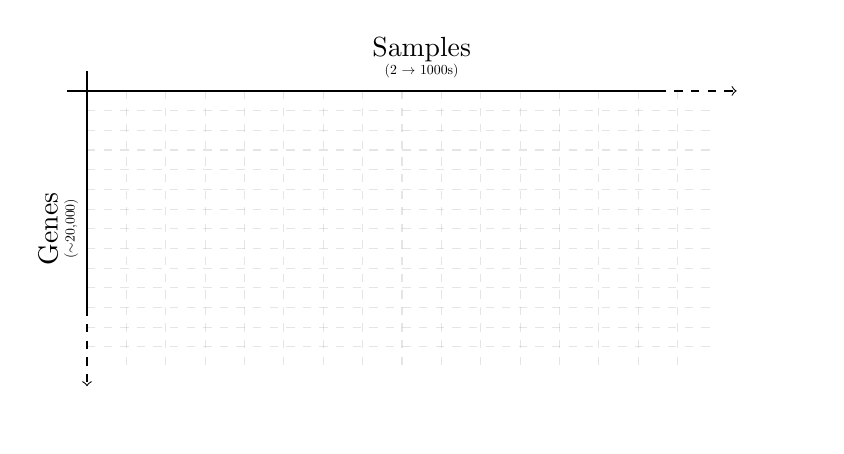
\begin{tikzpicture}[scale=0.5]
      \draw [help lines, opacity=0.0] (0,0) grid (20,10);
%      \foreach \x in {1,2,...,19} \node [font=\small] at (\x,0) {\x};
%      \foreach \y in {1,2,...,10} \node [font=\small] at (20,\y) {\y};
      \node [above] at (10,9) {Samples};
      \node [above, rotate=90] at (1,5) {Genes};
%      \draw [->] (9,8.75) node [left, font=\footnotesize] {(2}
%      -- (9.5,8.75) node [right, font=\footnotesize] {1000s)};
      \node [below, scale=0.5] at (10,9.3) {(2 $\rightarrow$ 1000s)};
      \node [below, rotate=90, scale=0.5] at (0.8,5) {($\sim$20,000)};
      \draw [-] (1,8.5) -- (16,8.5);
      \draw [-] (1.5,9) -- (1.5,3);
      \draw [->,dashed] (16,8.5) -- (18,8.5);
      \draw [->,dashed] (1.5,3) -- (1.5,1);
      \foreach \y in {8.0,7.5,...,2.0} \draw [-,opacity=0.1,dashed] (1.5,\y) -- (17.5,\y);
      \foreach \x in {2.5,3.5,...,16.5} \draw [-,opacity=0.1,dashed] (\x,8.5) -- (\x,1.5);
    \end{tikzpicture}
  \end{figure}
  \blfootnote{I really dislike the term transcriptomics}
  \blfootnote{And this is obviously rather over-simplified}
\end{frame}


\begin{frame}{other omics}
  May be considered later.
\end{frame}

\begin{frame}{Databases}
  A database is just a collection of data.
  \pause
  But can be structured in different ways.
  \begin{description}[Object orientated]
    \item[Flat file] Just a bunch of files.
    \item[Relational] Data structured by the definition of relationships.
    \item[Object orientated] Data structured into logical objects.
  \end{description}
  \pause
  The challenge is to represent reality in a flexible and structured manner that can provide
  guarantees about data integrity and that facilitate data modification.
  
  \pause
  How to structure data: useful lessons for labelling stuff and taking notes.
\end{frame}

\begin{frame}{Structures}
  The structure of both proteins and functional RNA molecules are directly related to how
  they work and are regulated.

  This is useful information, but difficult to obtain experimentally. Structures can sometimes
  be derived computationally.

  This can be considered a part of bioinformatics.
\end{frame}

\begin{frame}{Summary}
  \subHeading{The problem domain is biology}

  Biology is defined by information.
\end{frame}

\end{document}
